\section{Bahnplanung \robo{71}{4}}
\subsection{Bewegungsarten \robo{71}{4.1}}
\begin{minipage}{0.5\linewidth}
    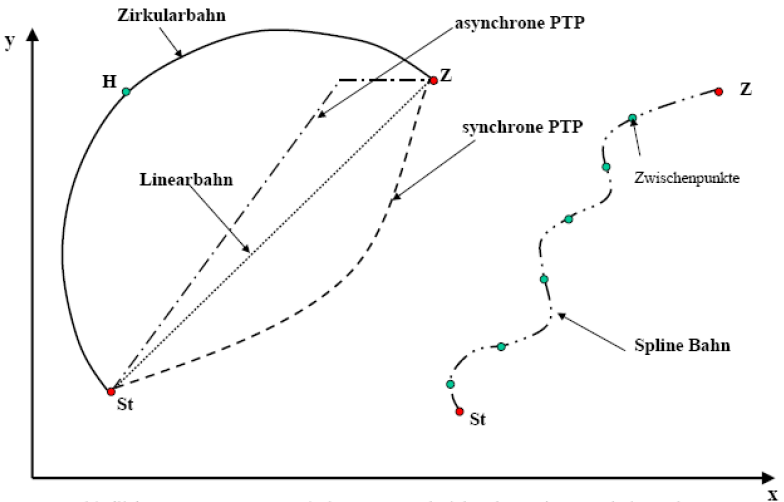
\includegraphics[width=0.9\linewidth]{./bilder/bewegungsarten}
\end{minipage}
\begin{minipage}{0.5\linewidth}
    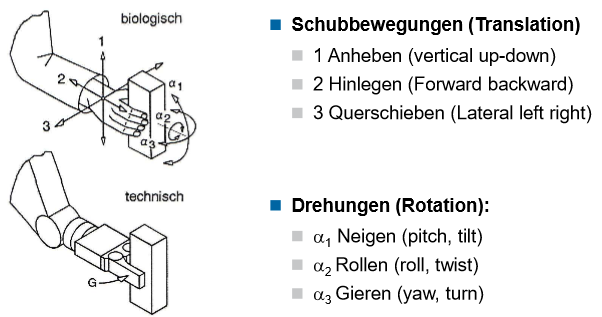
\includegraphics[width=\linewidth]{./bilder/BewegungGreifer}
\end{minipage}

\begin{minipage}{0.5\linewidth}
    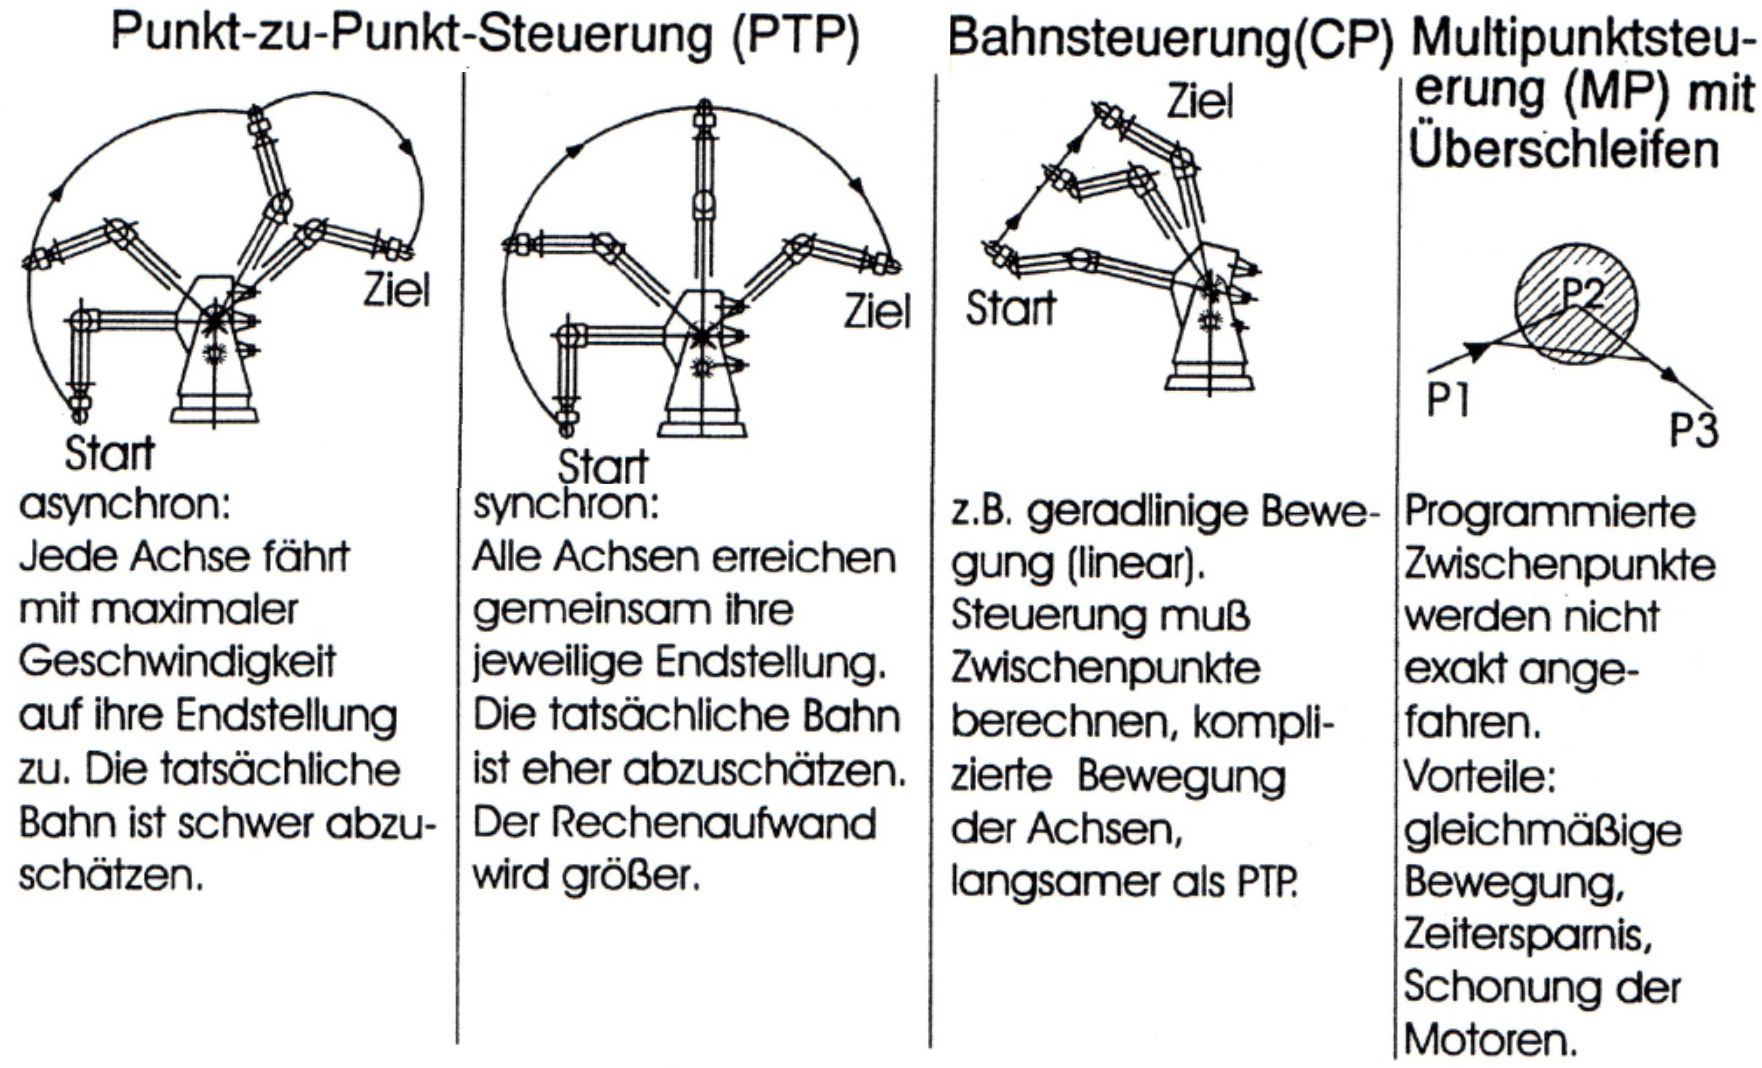
\includegraphics[width=\linewidth]{./bilder/bewegungsarten2}
\end{minipage}


\subsubsection{Singularität}
\begin{minipage}{0.5\linewidth}
    \textbf{Singuläre Konfiguration}
    \begin{itemize}
        \item Mehrere Achsen liegen in einer Linie
        \item Die Drehung einer Achse kann durch Gegendrehung einer anderen Achse kompensiert werden.
        \item Ein Freiheitsgrad geht verloren, da für eine Drehachse zwei Gelenke verwendet werden.
    \end{itemize}
\end{minipage}
\begin{minipage}{0.5\linewidth}
    \textbf{Grenzsingularität}\newline
    \begin{itemize}
        \item Der Roboter ist ganz ausgestreckt oder an einer Position am Rande seines Arbeitsraum
        \begin{itemize}
            \item Es gibt Richtungen in die er sich nicht mehr bewegen kann
        \end{itemize}
    \end{itemize}
\end{minipage}

\subsection{Bahnüberschleifen \robo{96}{4.4}}
Vorteile:
\begin{itemize}
    \item[+] Zeitgewinn
    \item[+] Vermeidung von ruckartigen Bewegungen
    \item[+] Hindernisumfahrung durch Definition von Zwischenpunkten 
\end{itemize}

\begin{minipage}{0.345\linewidth}
    \textbf{PTP} \robo{97}{4.4.1}\newline
    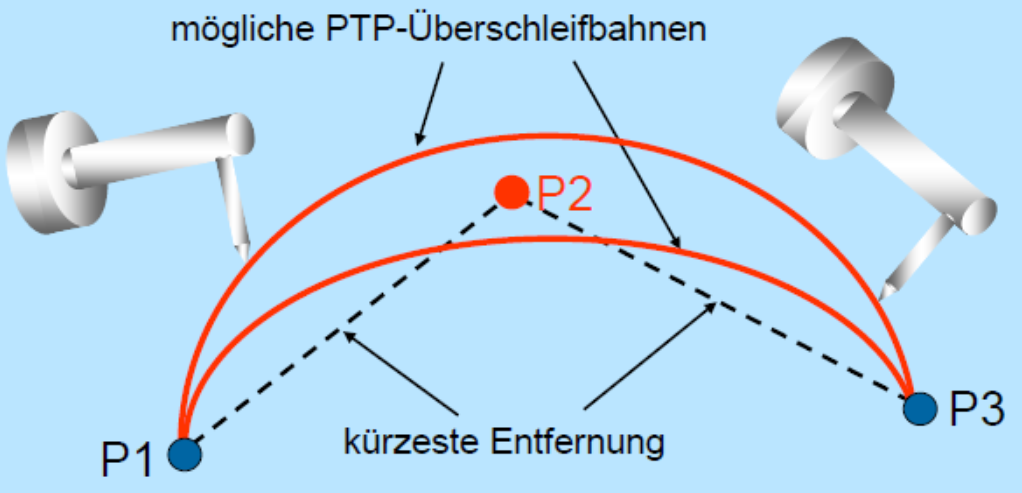
\includegraphics[width=\linewidth]{./bilder/UeberschleifenPTP}
\end{minipage}
\begin{minipage}{0.32\linewidth}
    \textbf{Linear}\robo{98}{4.4.2}\newline
    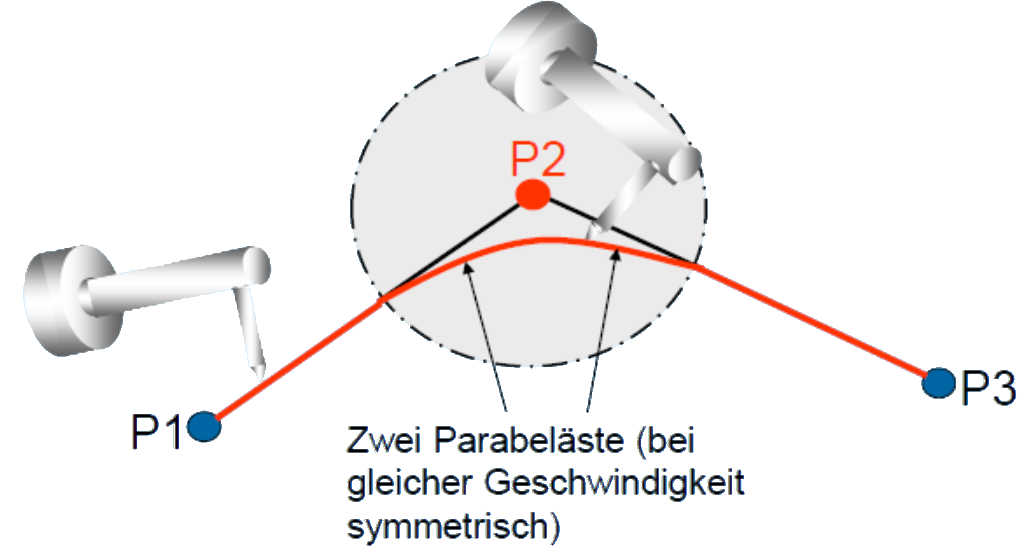
\includegraphics[width=\linewidth]{./bilder/UeberschleifenLin}
\end{minipage}
\begin{minipage}{0.32\linewidth}
    \textbf{Zirkular}\newline
    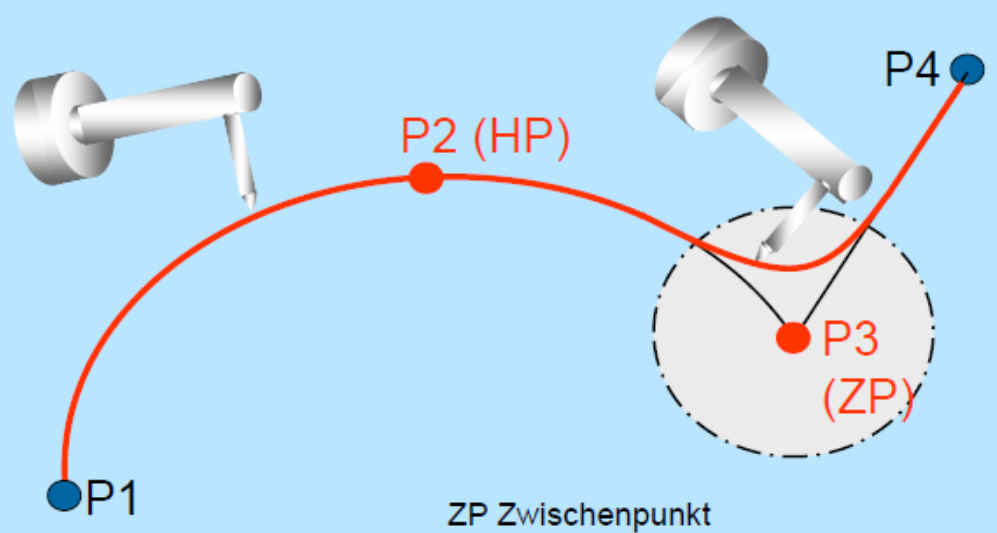
\includegraphics[width=\linewidth]{./bilder/UeberschleifenCirc}
\end{minipage}

\subsection{Bahnerzeugungn in Gelenkkoordinaten}
\begin{multicols}{2}
    \begin{itemize}
        \item[+] Minimale Bewegung bei jedem Gelenk.
        \item[+] Max. Geschwindigkeit und max. Momente bekannt.
    \end{itemize}

    \begin{itemize}
        \item[-] Bahngeometrie in kart. Raum unbekannt.
        \item[-] Kollisionsvermeidung schwierig.
    \end{itemize}
\end{multicols}
\clearpage
\subsubsection{Kubisches Polynom}
\begin{tabular}{ll}
\multicolumn{2}{l}{\textbf{Bedingungen}}\\
$ \theta(0)=\theta_0 $& $ \theta(t_f) = \theta_f$\\ 
$ \dot{\theta}(0)=0 $& $ \dot{\theta}(t_f) = 0$\\
\multicolumn{2}{l}{\textbf{Gleichung}}\\
\multicolumn{2}{l}{$ \theta(t)=a_0 + a_1t + a_2t^2+a_3t^3$}\\
\multicolumn{2}{l}{\textbf{Koeffizienten}}\\
$a_0= \theta_0$&$a_1=0 $\\
$a_2 = \frac{3}{t_f^2}(\theta_f - \theta_0) $&$a_3=-\frac{2}{t_f^3}(\theta_f-\theta_0) $\\
\end{tabular}
\paragraph{Bsp.}
Ein Roboter mit einer Rotationsachse ($\theta$) soll sich von $\theta$= -5\textdegree bis zu $\theta$= 80\textdegree in 4 Sekunden bewegen.\newline
Gesucht: Koeff des kubischen Polynoms, max Geschwindigkeit und max Beschleunigung der Achsen.
Stellen sie die Position Grafisch dar.

\begin{tabular}{ll}
    Kubisches Polynom & $\theta(t)=a_0 + a_1t + a_2t^2+a_3t^3$\\
                        & $a_0 = -5$\textdegree$,\; a_1=0,\; a_2=15.93,\; a_3=-2.656 $\\
    Geschwindigkeit     & $\dot{\theta}=a_1+2a_2\cdot t+3a_3 \cdot t^2 $\\
                        & $ \qquad 31.86 \cdot t - 7.968 \cdot t^2$\\
    Beschleunigung      & $ \ddot{\theta}=2a_2 + 6a_3 \cdot t$\\
                        & $ \qquad 31.86 - 15.936 \cdot t$\\
    $\rightarrow \ddot{\theta}=0 $ & t = $\frac{31.86}{15.936}=2s$\\
    max. Geschw.        & $ \dot{\theta}_{max}= 31.86\cdot 2s - 7.968\cdot 4s = 31.848$\textdegree$ /s$\\
    max. Besch.         &$ \ddot{\theta}_{max} \rightarrow t=0 $ \\  
                        &$ \ddot{\theta}_{max} \rightarrow t=t_f $ \\              
\end{tabular}

\clearpage
\subsubsection{Rampenprofil \robo{75}{4.2.2}}
\begin{minipage}{0.4\linewidth}
    \begin{align*}
        s_e &= |q_Z - q_{St}|\\
        t_b &= \frac{v_m}{b_m}\\
        t_e &= \frac{s_e}{v_m}+t_b\\
        t_v &= t_e - t_b = \frac{s_e}{v_m}
    \end{align*}
        \begin{tabular}{ll}
        $q_Z$ & Zielkoordinaten\\
        $q_{St}$& Startkoordinaten\\
        $t_b$ & Beschleunigungszeit\\
        $t_v$ & Bremszeitpunkt \\
        $t_e$ & Dauer der Bewegung\\
        $v_m$ & Bahngeschwindigkeit\\
        $b_m$ & Bahnbeschleunigung\\
        $s_e$ & Länge der Bahn\\
    \end{tabular}
\end{minipage}
\begin{minipage}{0.25\linewidth}
    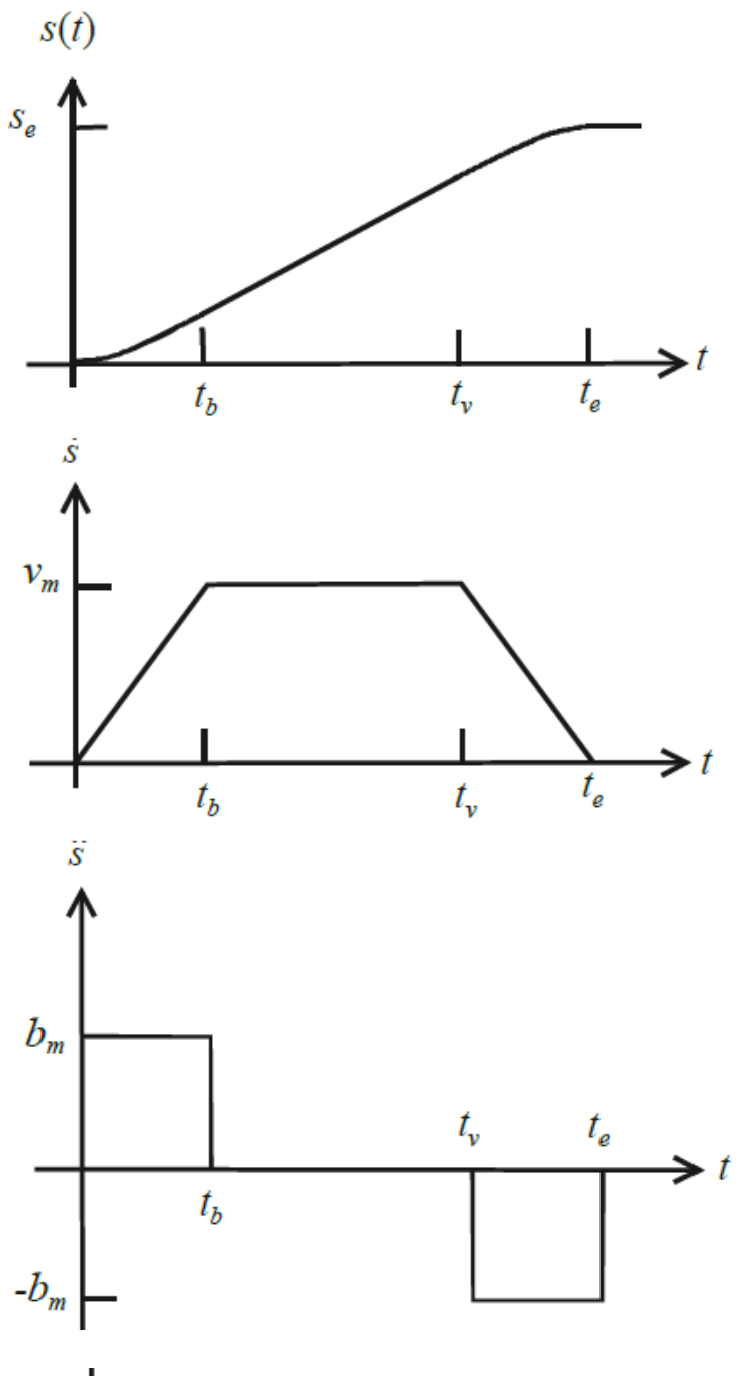
\includegraphics[width=\linewidth]{./bilder/RampenTrapez}
\end{minipage}
\begin{minipage}{0.35\linewidth}
    \textbf{Ablauf Korrektur\newline zeit-optimaler Bahn}\newline
    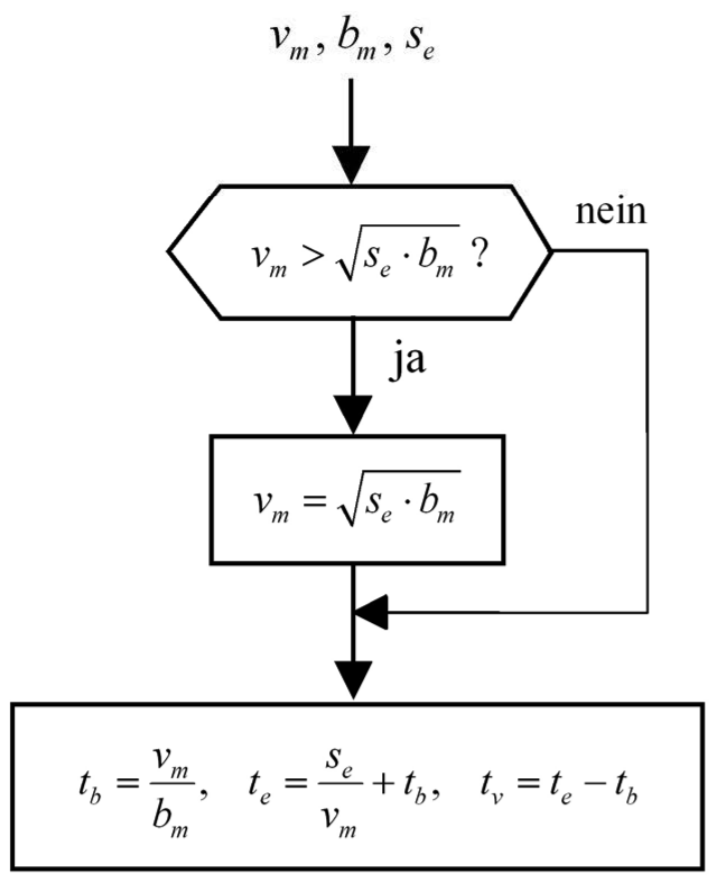
\includegraphics[width=\linewidth]{./bilder/RampenVorgehn}
\end{minipage}
    \begin{align*}
0 \le   &t \le t_b   &  \ddot{s}(t) &= b_m        & \dot{s}&=b_m \cdot t               &  s(t)&=\frac{1}{2}\cdot b_m \cdot t^2\\ 
t_b \le &t \le t_v   &  \ddot{s}(t) &= 0          &  \dot{s}&=v_m \cdot t              &  s(t)&=v_m \cdot t - \frac{1}{2}\cdot \frac{v_m^2}{b_m}\\
t_v \le &t \le t_e   &  \ddot{s}(t) &= -b_m       &  \dot{s}&=v_m -b_m \cdot (t-t_v)   &  s(t)&=v_m \cdot t_v - \frac{b_m}{2}\cdot(t_e - t)^2\\       
&            &              &             &  \dot{s}&=b_m \cdot (t_e-t)                &      &
\end{align*}
\begin{minipage}{0.5\linewidth}
    \textbf{BSP:}\newline
    {\small 
    Die Beschleunigung der Übergangsphase $\ddot{\theta}$ ist gegeben\newline
    \begin{align*}
        \ddot{\theta}\cdot t_b &= \frac{\theta_h-\theta_b}{t_h - t_b}\\
        \theta_b &=\theta_0 + \frac{1}{2}\ddot{\theta}\cdot t_b^2\\
        t_b &= \frac{t}{2}- \frac{\sqrt{t^2\cdot \ddot{\theta}^2-4\ddot{\theta}\cdot(\theta_f)- \theta_0}}{2\ddot{\theta}}\\
        t_h &= \frac{1}{2}t_f\\
        \theta_h &=\frac{1}{2}(\theta_f -\theta_0)
    \end{align*}
    \begin{tabular}{ll}
        $t_b$ & Länge des Übergangs\\
        $t_f$ & Dauer der Bewegung\\
        $t_h$ & \\
        $\theta_b$& Ende des Übergangs\\
        $\theta_h$& \\
        $\ddot{\theta}$& Beschleunigung während des Übergangs\\
    \end{tabular}}
\end{minipage}
\begin{minipage}{0.5\linewidth}
    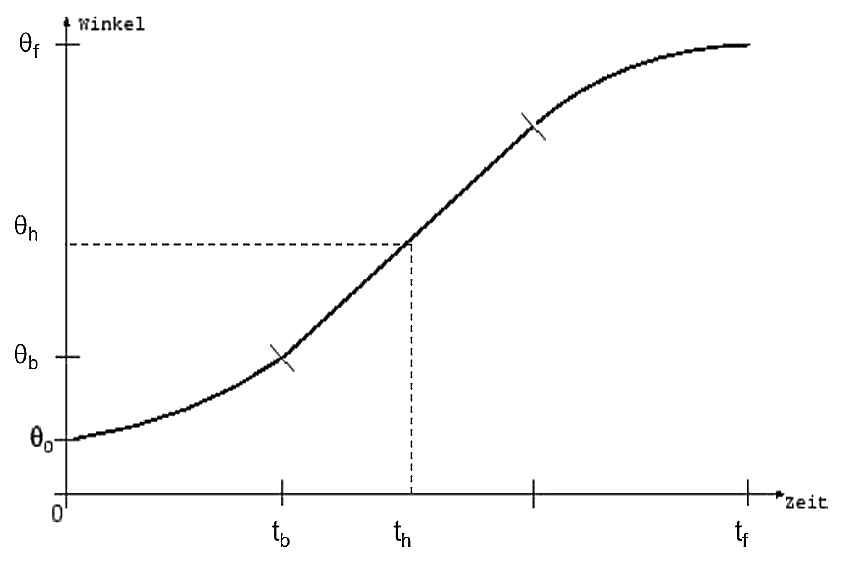
\includegraphics[width=0.9\linewidth]{./bilder/RampenprofilInterpol}
\end{minipage}
\clearpage
\subsubsection{Bahn mit Zwischenpunkten}
\begin{minipage}{0.5\linewidth}
    \begin{align*}
    \dot{\theta}_{jk} &= \frac{\theta_k - \theta_j}{t_{djk}}\\
    \ddot{\theta}_{jk} &= SGN(\dot{\theta}_{kl}-\dot{\theta}_{jk})|\ddot{\theta}_k|\\
    t_k &= \frac{\dot{\theta}_{kl}- \dot{\theta}_{jk}}{\ddot{\theta}_k}\\
    t_{jk}&=t_{djk}-\frac{1}{2}t_j - \frac{1}{2}t_k\\
    \end{align*}
    Allgemein:
    \begin{align*}
    \dot{\theta}_{(n-1)n} &= \frac{\theta_n - \theta_{n-1}}{t_{d(n-1)n}-\frac{1}{2}t_n}\\
    \ddot{\theta}_n &= SGN(\dot{\theta}_{n-1}-\dot{\theta}_{n})|\ddot{\theta}_n|\\
    t_n &= t_{d(n-1)n}-\sqrt{t^2_{d(n-1)n}+\frac{2(\theta_n - \theta_{n-1})}{\ddot{\theta}_n}}\\
    t_{(n-1)n} &= t_{d(n-1)n}-t_n - \frac{1}{2}t_{n-1}\\
    \end{align*}
\end{minipage}
\begin{minipage}{0.5\linewidth}
    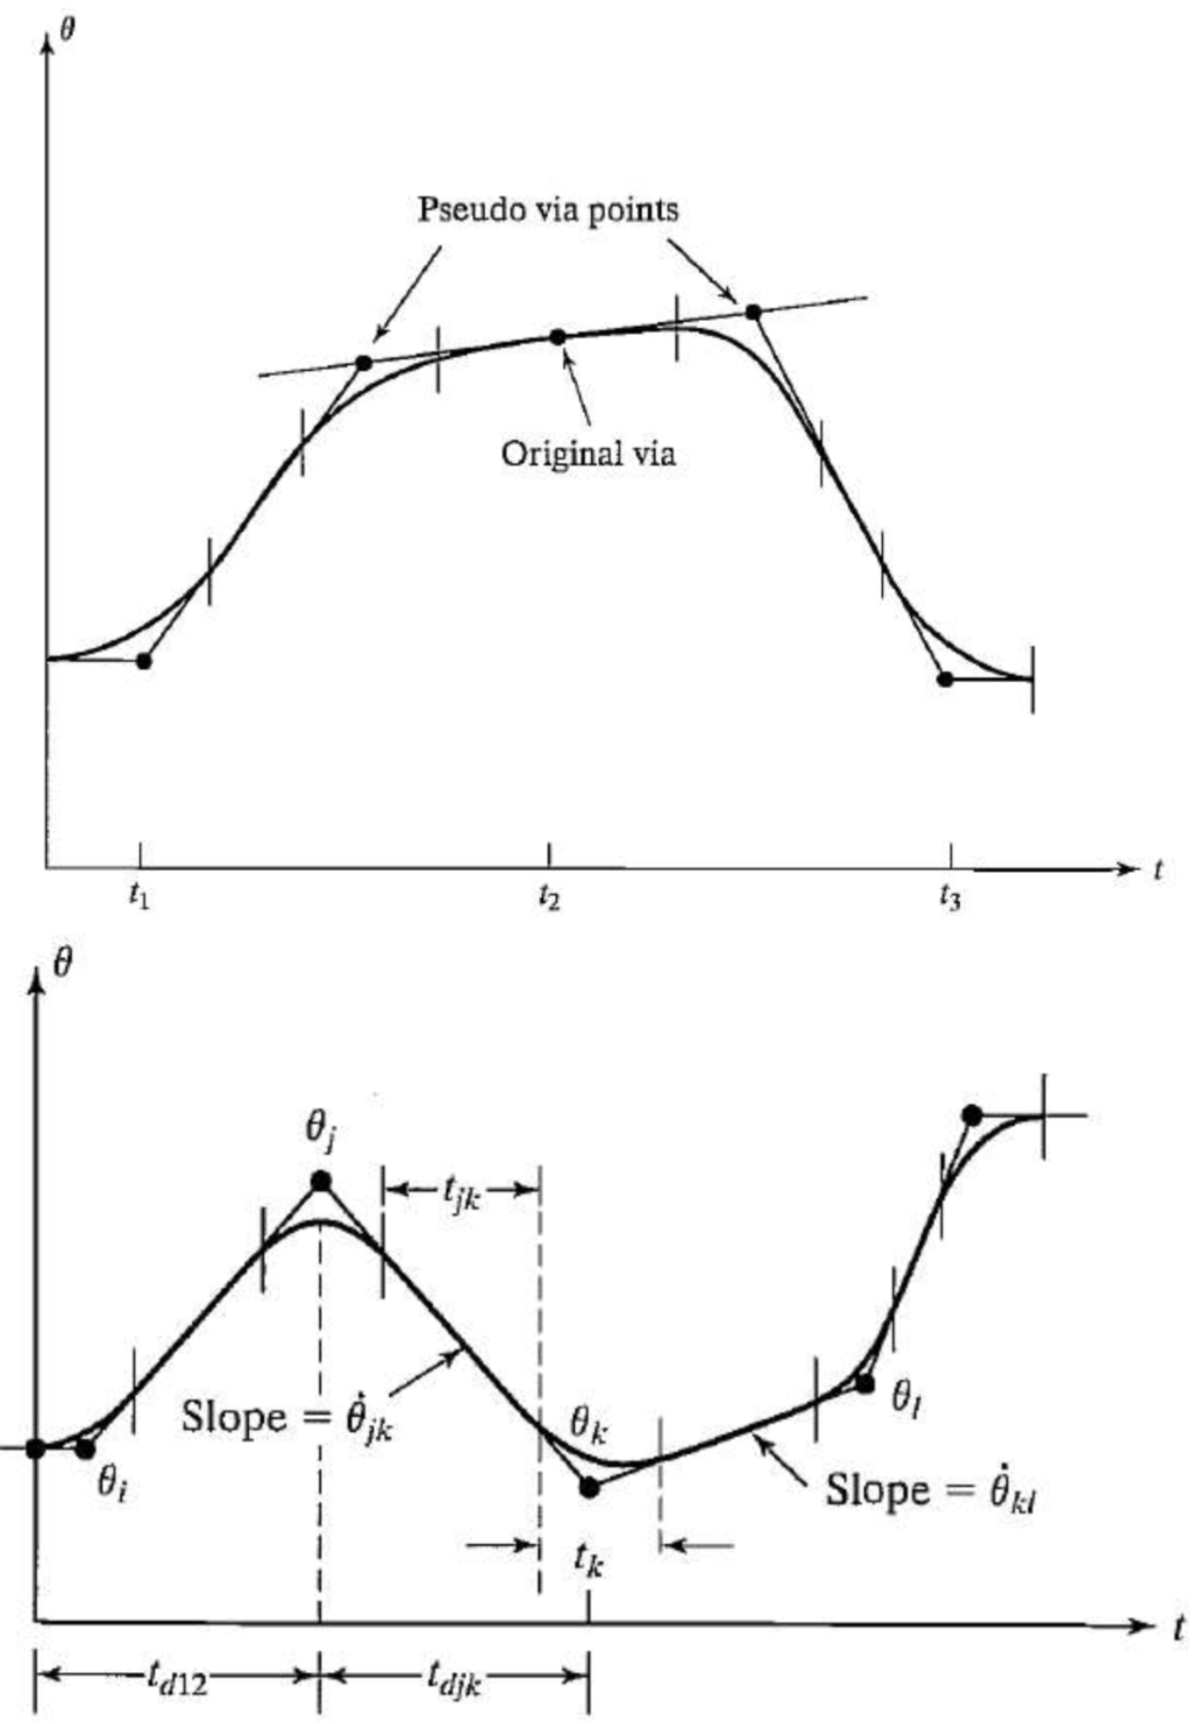
\includegraphics[width=0.9\linewidth]{./bilder/BahnMitZP}
\end{minipage}
\clearpage
\subsection{Interpolationsschrittweite \robo{79}{4.2.4}}
\subsection{PTP-Synchronisierung}
\begin{minipage}{0.7\linewidth}
    \begin{itemize}
        \item  \textbf{asynchronen PTP}
        \begin{itemize}
            \item  Jede Achse verfährt vollständig unabhängig von anderen Achsen.
        \end{itemize}
    \item[]
        \item  \textbf{synchronen PTP \robo{81}{4.2.5}}
        \begin{itemize}
            \item  Wird durch die Achse mit der grössten Bahndauer bestimmt.
            \item Die Geschwindigkeit der anderen Achsen wird reduziert,so dass alle gleichzeitig ihren Endpunkt erreichen.
        \end{itemize}
    \item[]
        \item  \textbf{vollsynchronen PTP \robo{82}{4.2.6}}
        \begin{itemize}
            \item  Nicht nur die Bahnzeiten für die Gelenke synchronisiert.
            \item Auch Beschleunigungs und Bremezeiten synchron.
        \end{itemize}
    \end{itemize}
\end{minipage}
\begin{minipage}{6cm}
    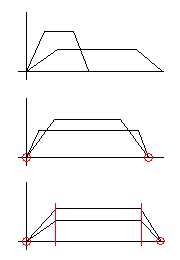
\includegraphics[width=5cm]{./bilder/synchron}
\end{minipage}
\newline
\subsubsection{synchrone PTP \robo{81}{4.2.5}}
\textbf{Vorgehen:}\newline \vspace{-\baselineskip}
\begin{itemize}
    \item Wie bei der asynchronen PTP zuerst $s_{e,i}$, $ v_{m,i}$, $b_{m,i}$ und $t_{e,i}$ bestimmen. (Bsp. mit Rampenprofil)
    \item Maximale Fahrzeit ermitteln: $t_e=max(t_{e,i})$.
    \begin{itemize}
        \item Achse mit der max. Fahrzeit ist die \textbf{Leitachse}
    \end{itemize} 
    \item Für alle Gelenke gilt: $t_{e,i}=t_e$
    \item Geschwindigkeit der Gelenke $v_{m,i}$, welche nicht die Leitgelenke sind werden angepasst
\end{itemize}
\[ t_e=\frac{s_{e,i}}{v_{m,i}}+\frac{v_{m,i}}{b_{m,i}}  \quad \rightarrow \quad 
 v_{m,i}=\frac{b_{m,i}\cdot t_e}{2}- \sqrt{\frac{b_{m,i}^2\cdot t_e^2}{4}-s_{e,i}\cdot b_{m,i}} \]
Wegen $t_e \ge 2\cdot t_{b,i}$ ist nur der kleiner Wert sinnvoll.
\subsubsection{vollsynchrone PTP \robo{82}{4.2.6}}
\textbf{Vorgehen:}\newline \vspace{-\baselineskip}
\begin{itemize}
    \item Wie bei synchron PTP \textbf{Leitachse} bestimmen.
    \begin{itemize}
        \item Gibt $t_e$, $t_b$ und $t_v=t_e-t_b $ vor.
    \end{itemize}
    \item Geschwindigkeit und Beschleunigung der Gelenke $v_{m,i}$, welche nicht die Leitgelenke sind werden angepasst
\end{itemize}    
\[ v_{m,i}= \frac{s_{e,i}}{t_v} \qquad b_{m,i}=\frac{v_{m,i}}{t_b} \]

\subsection{Vergleich Bahnverläufe \robo{83}{4.2.7}}
\begin{multicols}{3}
    \begin{minipage}{\linewidth}
        \subsubsection{Asynchroner PTP}
        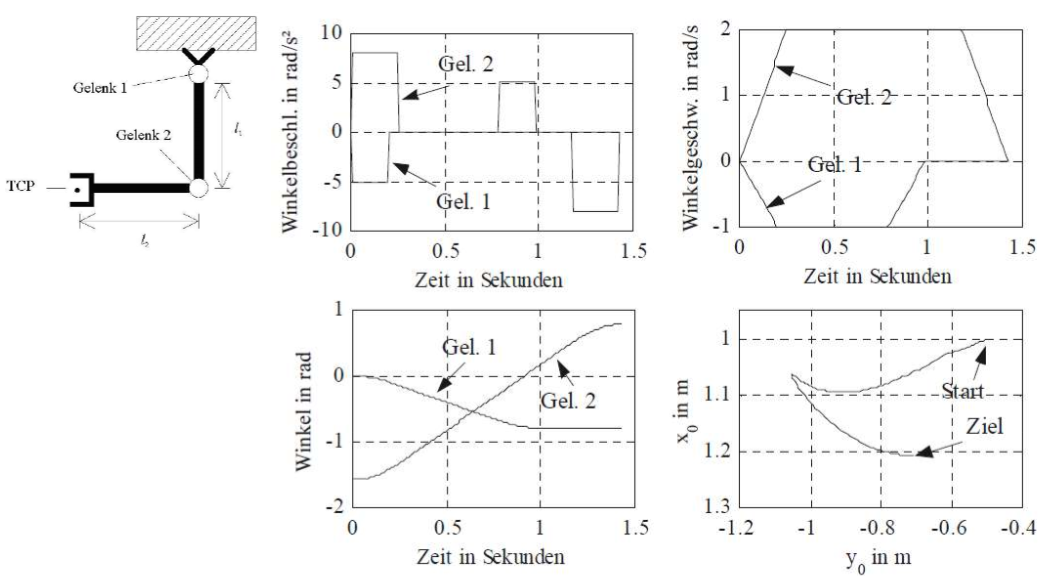
\includegraphics[width=\linewidth]{./bilder/VBAPTP}
    \end{minipage}
    
    \begin{minipage}{\linewidth}
        \subsubsection{Voll-synchroner PTP}
        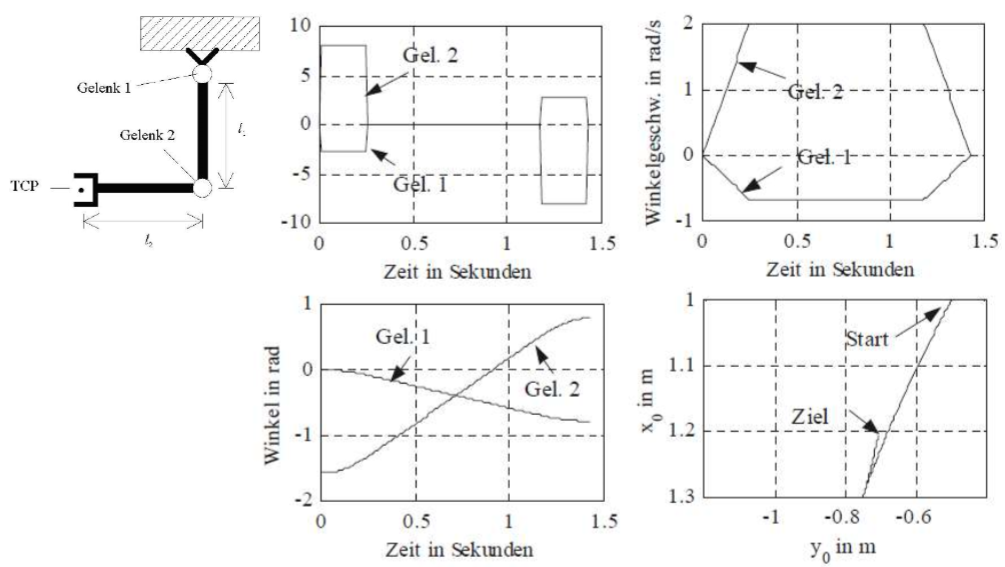
\includegraphics[width=\linewidth]{./bilder/VBVPTP}
    \end{minipage}
    
    \begin{minipage}{\linewidth}
        \subsubsection{CP-Bahn (linear)}
        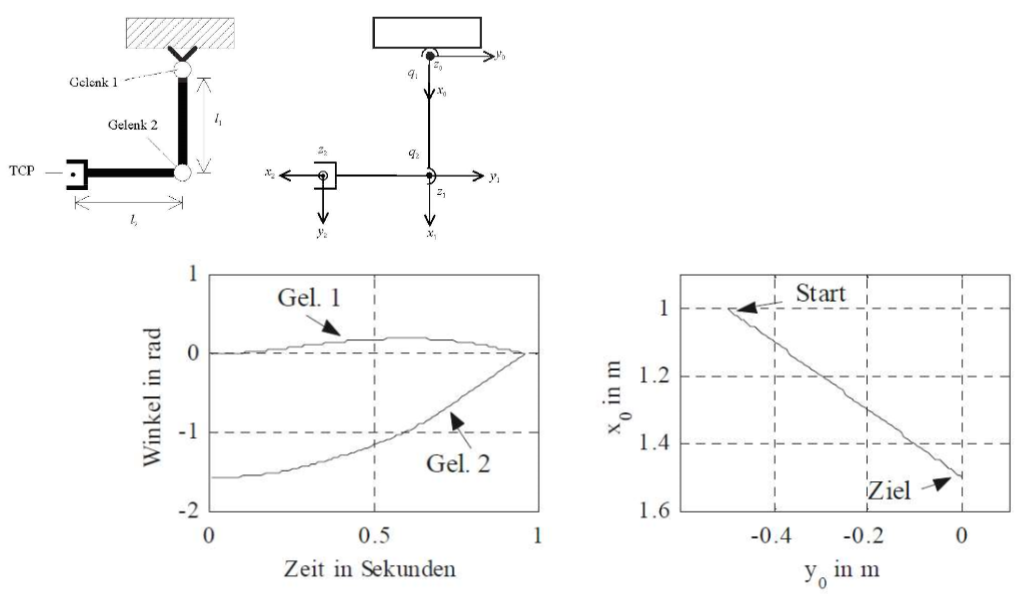
\includegraphics[width=\linewidth]{./bilder/VBCPB}
    \end{minipage}
\end{multicols}
\clearpage  %========================================================================
\subsection{Bahnerzeugungn in karteschien Koordinaten / Bahnsteuerung \robo{85}{4.3}}
\begin{multicols}{2}
    \begin{itemize}
        \item[+] Bahn genau definiert
    \end{itemize}
    
    \begin{itemize}
        \item[-] Berechnung der inv. Koordtrans für jeden Punkt notwendig.
        \item[-] Schwierig, die Motorenbegrenzung zu berücksichtigen.
        \columnbreak
        \item[-] Geometrische Probleme
        \begin{itemize}
            \item Unerreichbare Zwischenpunkte
            \item Hohe v in der Nähe von Singularitäten
            \item Start/Ziel gehören zu verschiedenen Zweige der kin. Lösung
        \end{itemize}
    \end{itemize}
\end{multicols}

\begin{minipage}{0.5\linewidth}
\begin{itemize}
    \item Der TCP bewegt sich auf einer Geraden zur Zielposition
    \begin{itemize}
        \item Interpolation für TCP im Raum
    \end{itemize}
\item Die Orientierung kann ändern
\begin{itemize}
    \item Interpolation für Euler-Winkel
\end{itemize}
\item Unterscheidung einer synchronen und asynchronen Bahn ist nicht notwendig da normalerweise alle Gelenke an der Bewegung beteiligt sind.
\end{itemize}
\end{minipage}
\begin{minipage}{0.5\linewidth}
    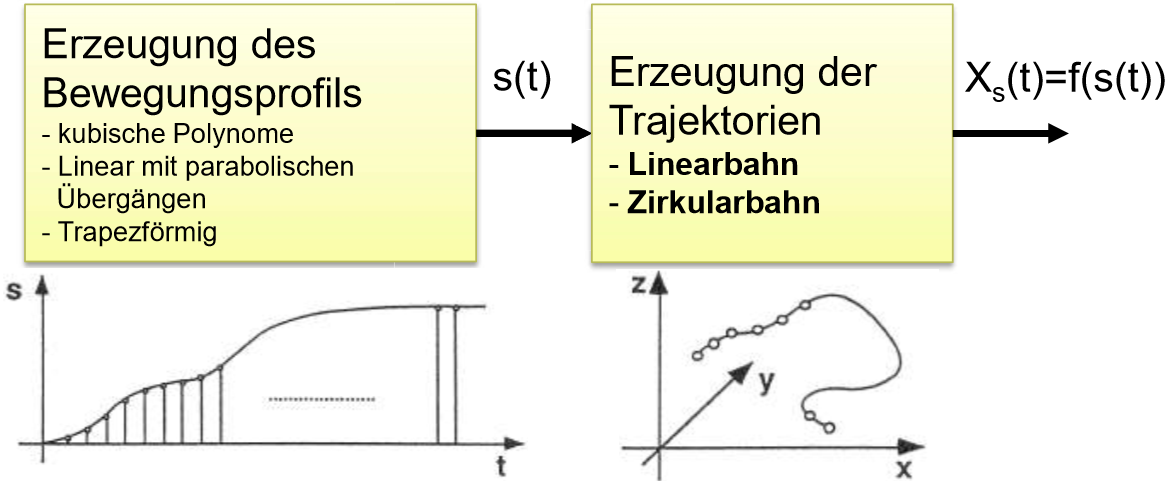
\includegraphics[width=\linewidth]{./bilder/Bahnsteuerung}
\end{minipage}

\begin{minipage}{0.7\linewidth}
    \subsubsection{Lineare Interpolation \robo{86}{4.3.2}}
    \vspace{-0.8cm}
    \[ X_s(t) = X_0 + s(t) \cdot u \]
    \[ u= \frac{x_f - x_0}{||x_f -x_0||} \rightarrow \text{Richtungsvektor}\]
    \[ s(t)=a_0 + a_1 t + a_2 t^2 +a_3t^3 \]
    \[ a_0=0 \quad a_1=0 \quad a_2=\frac{3\cdot ||x_f-x_0||}{t_f^2} \quad a_3=-\frac{2}{t_f^3}\cdot ||x_f-x_0||  \]
\end{minipage}
\begin{minipage}{0.3\linewidth}
    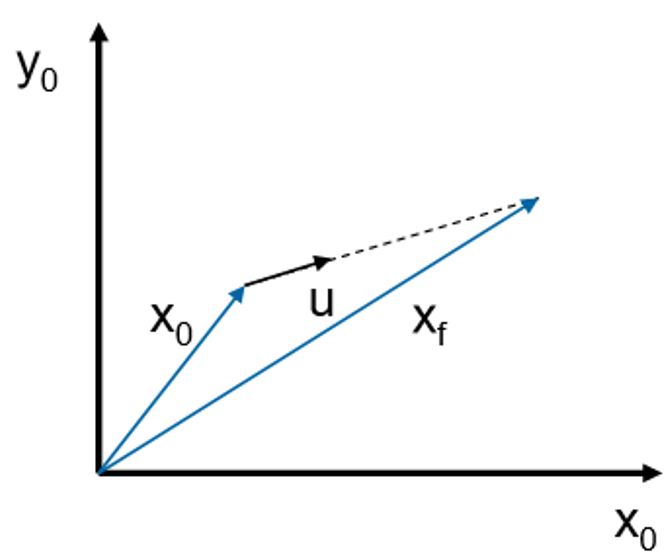
\includegraphics[width=0.9\linewidth]{./bilder/LinInter}
\end{minipage}

\subsubsection{Zirkulare Interpolation \robo{88}{4.3.3}}
\clearpage

